\documentclass[review]{elsarticle}

\usepackage{lineno}
\usepackage{makecell}
\usepackage[hidelinks]{hyperref}
\hypersetup{
    colorlinks,
    linkcolor={blue!50!black},
    citecolor={blue!50!black},
    urlcolor={blue!50!black}
}
%\modulolinenumbers[5]

\journal{International Journal of Heat and Fluid Flow}

%%%%%%%%%%%%%%%%%%%%%%%
%% Elsevier bibliography styles
%%%%%%%%%%%%%%%%%%%%%%%


%% `Elsevier LaTeX' style
\bibliographystyle{elsarticle-num}
%%%%%%%%%%%%%%%%%%%%%%%

\usepackage{xcolor}
\usepackage{float}
\usepackage{amsmath}

\usepackage{setspace}
\biboptions{sort&compress}
\setlength{\bibsep}{4pt}

\setlength{\abovecaptionskip}{-2pt plus 0pt minus 0pt}
\setlength{\belowcaptionskip}{2pt plus 0pt minus 0pt}

\newcommand{\ave}[1]{\left<{#1}\right>}

\begin{document}

\begin{frontmatter}

\title{On the Validations and Verifications of Lattice Boltzmann Simulation of a Single Bubble based on  Rayleigh-Plesset Equation}


%% or include affiliations in footnotes:
\author[address_1]{Xin Xiong}
\author[address_1]{Tom-Robin Teschner\corref{mycorrespondingauthor}}
\cortext[mycorrespondingauthor]{Corresponding author}
\ead{tom.teschner@cranfield.ac.uk}
\author[address_1]{Irene Moulitsas}
\author[address_1]{Tam\'{a}s Istv\'{a}n J\'{o}zsa}


\address[address_1] { Centre for Computational Engineering Sciences, Cranfield University, Cranfield MK43 0AL, UK.}

\begin{abstract}
This article validates the R-P equation based on LBM simulation against a single bubble. In addition, SINDy algorithm is used to replicate R-P terms. Firstly, a two-dimensional single bubble simulation is performed based on the Shan-Chen model with velocity shifting model and C-S equation of state. Laplace law and Maxwell area construction were then validated in this article to verify surface tension and thermal consistency validation. The validation of R-P equation is then performed. The results showed that after certain iterations the LBM simulation results start to deviate from the R-P equation, which may be due to the fact that the resolution of the bubble is not large enough for collapse cases and the impact of boundary for the growth cases. It was also shown that with the increase of domain size, iterations where deviation larger than 5\% becomes larger. This also holds for a radius where deviation reaches 5\%. When the same terms of R-P are fed to SINDy algorithm customised library, and the same coefficient of R-P equation is implemented for initial guess, SINDy can provide similar results of coefficient with deviation less than 50\% in most cases. The same results in the middle of the data can provide a good match based on SINDy proving again that at the beginning and the end of the LBM simulation, it is not perfect. The novelty of this article is using SINDy to replicate the R-P equation based on LBM simulation data.
\end{abstract}

\begin{keyword}
Lattice Boltzmann Simulation, Rayleigh-Plesset Equation, Single Bubble, Sparse identification of non-linear dynamics (SINDy) algorithm
\MSC[2010] 76D55
\end{keyword}


\end{frontmatter}

\linenumbers

%%%%%%%%%%%%%%%%%%%%%%%%%%%%%%%%%%%%%%%%%%%%%%%%%%%%%%%%%%%%%%%%%%%%%%
\section{Introduction}
\subsection{Background}
Cavitation is a phenomenon that includes liquid-to-vapour transition because of the decrease of pressure, which forms the number of vapour bubbles among liquids. It occurs in many hydrodynamic machines such as a propeller, the collapse of the cavitation bubble can cause high pressure and high temperature which is the reason for noise, vibration,and erosion.This may makes the machine worse performance or even break \cite{peng2019simulation}. However, cavitation can be taken advantage of for enhancing heat transfer or chemical reaction, such as sonochemistry \cite{thompson1999sonochemistry}. 

Many numerical attempts have been made to simulate the cavitation bubble based on traditional macroscopic method by the Navier-Stokes equation \cite{ogloblina2018simulation,shang2022investigation,koch2016numerical}. In addition, because of its advantages in simulating the multiphase model for its simplicity and locality, LBM (Lattice Boltzmann Method) was also applied in cavitation bubble simulation. In particular, the multiphase LBM method is a diffusive interface method that is not necessary to track the interface explicitly. There are normally three models of multiphase LBM, which are the colour-gradient model, the Shan-Chen model, and the free energy model \cite{sudhakar2020evolution}.
\subsection{literature review}
Among all the multiphase LBM, the Shan-Chen model is quite popular in simulating bubble dynamics. For example, there are a lot of articles that study the single bubble near a solid wall based on the Shan-Chen model \cite{liu2021study,袁晓龙2020numerical,mao2018study}. In addition, other simulation of a bubble such as a single bubble near a concave wall \cite{shan2021investigation}, and a bubble near a solid particle \cite{peng2020simulation} was also performed. In these articles, the validation of bubble growth or collapse was all conducted by comparing the Rayleigh-Plesset (R-P) equation and the LBM simulation results. Shi et al. \cite{shi2020numerical} compare R-P equation with LBM simulation results from radius 20 that grows. The modified R-P equation with the impact of other bubbles is also validated from radius 20. Ezzatneshan and Vaseghnia \cite{ezzatneshan2021dynamics} also validated the LBM results of the same radius against R-P equation with different pressures. The critical pressure was obtained at which the bubble can either grow or collapse. Peng et al. \cite{peng2019simulation} compare the results of variable boundary pressure results of LBM against related R-P equation. The results showed good agreement but slight deviation at the beginning. Peng et al. \cite{peng2018single} study the results of LBM with different pressure differences and radius against the related R-P equation for two-dimensional cases. The results are good at certain parts of the iterations but some small deviations exist. 
Although the validation of R-P is performed in these studies, the impact of domain size, the location of where the comparison starts, the initial radius of the bubble, and the impact of the boundary condition of the LBM were not studied. 
\subsection{aims and article structures}
In this article, a different initial radius of bubbles with different domain sizes with a simple bounce-back boundary condition was simulated by the Shan-Chen LBM model. The detailed validation with the R-P equation was conducted to give insight into the impact of domain size, initial radius of the bubble and boundary condition on the accuracy of the simulation. Furthermore, a different equation closer to LBM results was tried to recover by SINDy algorithm.    

%%%%%%%%%%%%%%%%%%%%%%%%%%%%%%%%%%%%%%%%%%%%%%%%%%%%%%%%%%%%%%%%%%%%%%
\section{Methods}

\subsection{Equations of the Simulation}
In this project, a two-dimensional $D2Q9$ model was implemented based on the Shan-Chen multiphase model. The additional force was considered based on the velocity shifting method by changing the equilibrium velocity without any modification of the Lattice Boltzmann Equation, which can be expressed as \cite{kruger2017lattice}
\begin{linenomath*}
\begin{equation}
	f_i\left(x+e_i \Delta t, t+\Delta t\right)-f_i(x, t)=-\frac{1}{\tau}\left[f_i(x, t)-f_i^{e q}(x, t)\right],
\end{equation}
\end{linenomath*}
The equilibrium density distribution function can be expressed as \cite{mohamad2011lattice}
\begin{linenomath*}
\begin{equation}
	f_i^{e q}(x, t)=\omega_i \rho(x)\left[1+\frac{3 \boldsymbol{e}_i \cdot \boldsymbol{u}}{c^2}+\frac{9\left(\boldsymbol{e}_i \cdot \boldsymbol{u}\right)^2}{2 c^4}-\frac{3 \boldsymbol{u}^2}{2 c^2}\right],
\end{equation}
\end{linenomath*}
where the weights $\omega_i$ equals 4/9 ($i$= 0), 1/9 ($i$= 1-4), 1/36 ($i$= 5-9). According to Shan and Chen \cite{shan1993lattice} the additional force can be expressed as
\begin{linenomath*}
\begin{equation}
	F(x, t)=-G \psi(x, t) \sum_{i=0}^8 \omega_i \psi\left(x+e_i t, t\right) e_i,
\end{equation}
\end{linenomath*}
where $G$ indicates the interaction strength between particles and $\psi$ is the effective density. In addition, the velocity shifting method was implemented because of stability \cite{kruger2017lattice} as
\begin{linenomath*}
\begin{equation}
	\boldsymbol{u}^{\mathrm{eq}}=\frac{1}{\rho}\left(\sum_i f_i \boldsymbol{c}_i+\tau \boldsymbol{F}\right).
\end{equation}
\end{linenomath*}
Furthermore, the C-S equation of state is incorporated by changing the effective density \cite{shi2020numerical}
\begin{linenomath*}
\begin{equation}
	\psi=\sqrt{\frac{2}{G c_s^2}\left(p-\rho c_s^2\right)},
\end{equation}
\end{linenomath*}
with different pressure. The C-S equation of state \cite{peng2019simulation}
\begin{linenomath*}
\begin{equation}
	P=\rho R T \frac{1+b \rho / 4+(b \rho / 4)^2-(b \rho / 4)^3}{(1-b \rho / 4)^3}-a \rho^2,
\end{equation}
\end{linenomath*}
is implemented in this project with $a= 0.4963R^2T_c^2/P_c$,$b=0.18727RT_c^2/P_c$. Where $ a= 1, b= 4, R= 1$, the
critical temperature, pressure and density are $T_c = 0.09433, P_c=0.00441644$, and $\rho_c= 0.13044$. In this project,$T/T_c$ is set to 0.75, and the simulation is assumed to be isothermal.

In addition, because in this project, the LBM simulation is a two-dimensional problem in a square domain so that the related R-P equation is derived based on cylindrical coordinate system from continuity, momentum equation and can finally be expressed as
\begin{linenomath*}
\begin{equation}
	\ddot{R}=\left(\frac{P_v-P_{\infty}}{\rho_l}-\frac{\sigma}{\rho_l R} -\frac{2 \nu}{R} \dot{R}+\frac{1-\left(\frac{R}{R \infty}\right)^2}{2} \dot{R}^2-\ln \frac{R_{\infty}}{R} \dot{R}^2\right)/\left(\ln \frac{R_{\infty}}{R} \cdot R\right),
\label{equ:r-p}
\end{equation}
\end{linenomath*}
where $R$, $R_{\infty}$,$\dot{R}$,$\ddot{R}$,$\sigma$,$\nu$,$\rho_l$,$P_v$,$P_{\infty}$ are radius, the distance between the centre of the domain and the boundary, first derivative of the radius, second derivative of the radius, the surface tension, kinematic viscosity, liquid density, vapour pressure and pressure on the boundary. Furthermore, to go to a further step, the non-dimensionless form of related R-P equation is also derived and listed here for reference as follows,
\begin{linenomath*}
\begin{equation}
	\begin{aligned}
		& \left(\ln \frac{R_{\infty}}{R^* L_{r e f}} \cdot R^*\right) \frac{d^2 R^*}{d t^{* 2}}= 
		 \frac{P_v-P_{\infty}}{\rho_l} \frac{L_{r e f}^2}{\nu^2}-\frac{\sigma}{\rho_l R^*} \frac{L_{r e f}}{\nu^2}-\frac{2}{R^*} \frac{d R^*}{d t *}+\\
		 &\frac{1-\left(\frac{R^* L_{r e f}}{R \infty}\right)^2}{2}\left(\frac{d R^*}{d t^*}\right)^2-\ln \frac{R_{\infty}}{R^* L_{r e f}}\left(\frac{d R^*}{d t^*}\right)^2,
	\end{aligned}
\end{equation}
\end{linenomath*}
where the same terminology with R-P equation is applied and  $L_{ref}$ is the reference length of the problem.
\subsection{Problem statement and the cases}
In this project, a single bubble was simulated based on the Shan-Chen model stated before, the equilibrium density of the liquid and gas was taken from Maxwell area construction based on C-S EOS and they are 0.33 and 0.011 respectively. For stability reasons, the reduced temperature was chosen to be 0.75 in this project. To trigger the growth and collapse of the bubble, a different density from the equilibrium density of liquid on the boundary was implemented which are 0.34 and 0.31 for collapse and growth respectively which is displayed in Figure \ref{fig:schematics}. In addition, for simplicity, the bounce-back boundary condition was implemented in this project. In addition, the interaction strength $G$ cannot affect the results since it will be eliminated during the calculation \cite{shi2020numerical} so it was set to -1 for simplicity, relaxation frequency $\omega$ is set to $1$ for a reason of good stability. Furthermore, 1000 time steps were simulated for a long enough time for bubble growth and collapse. The domain size for the bubble simulation is set to be a square from 100 to 1000. According to Peng et al \cite{peng2019simulation}, an initial smooth thickness of 5 lattices was set for better stability.
\begin{linenomath*}
\begin{equation}
	\begin{aligned}
		&\rho(y)=\rho_{\text {vapor }}+\\
		&\frac{\rho_{\text {liquid }}-\rho_{\text {vapor }}}{2}\left[\tanh \left(\frac{2(y-20)}{d}\right)-\tanh \left(\frac{2(y-20)}{d}\right)\right].
	\end{aligned}
\end{equation}
\end{linenomath*}

In this project, the Laplace Law and Maxwell area construction was first validated. To validate the Laplace Law, a periodic boundary condition was implemented, and three radii 20,25,30 with 100 domain size was set. The other settings are the same as the previous case settings. 

\begin{figure}[htp]
	\centering
	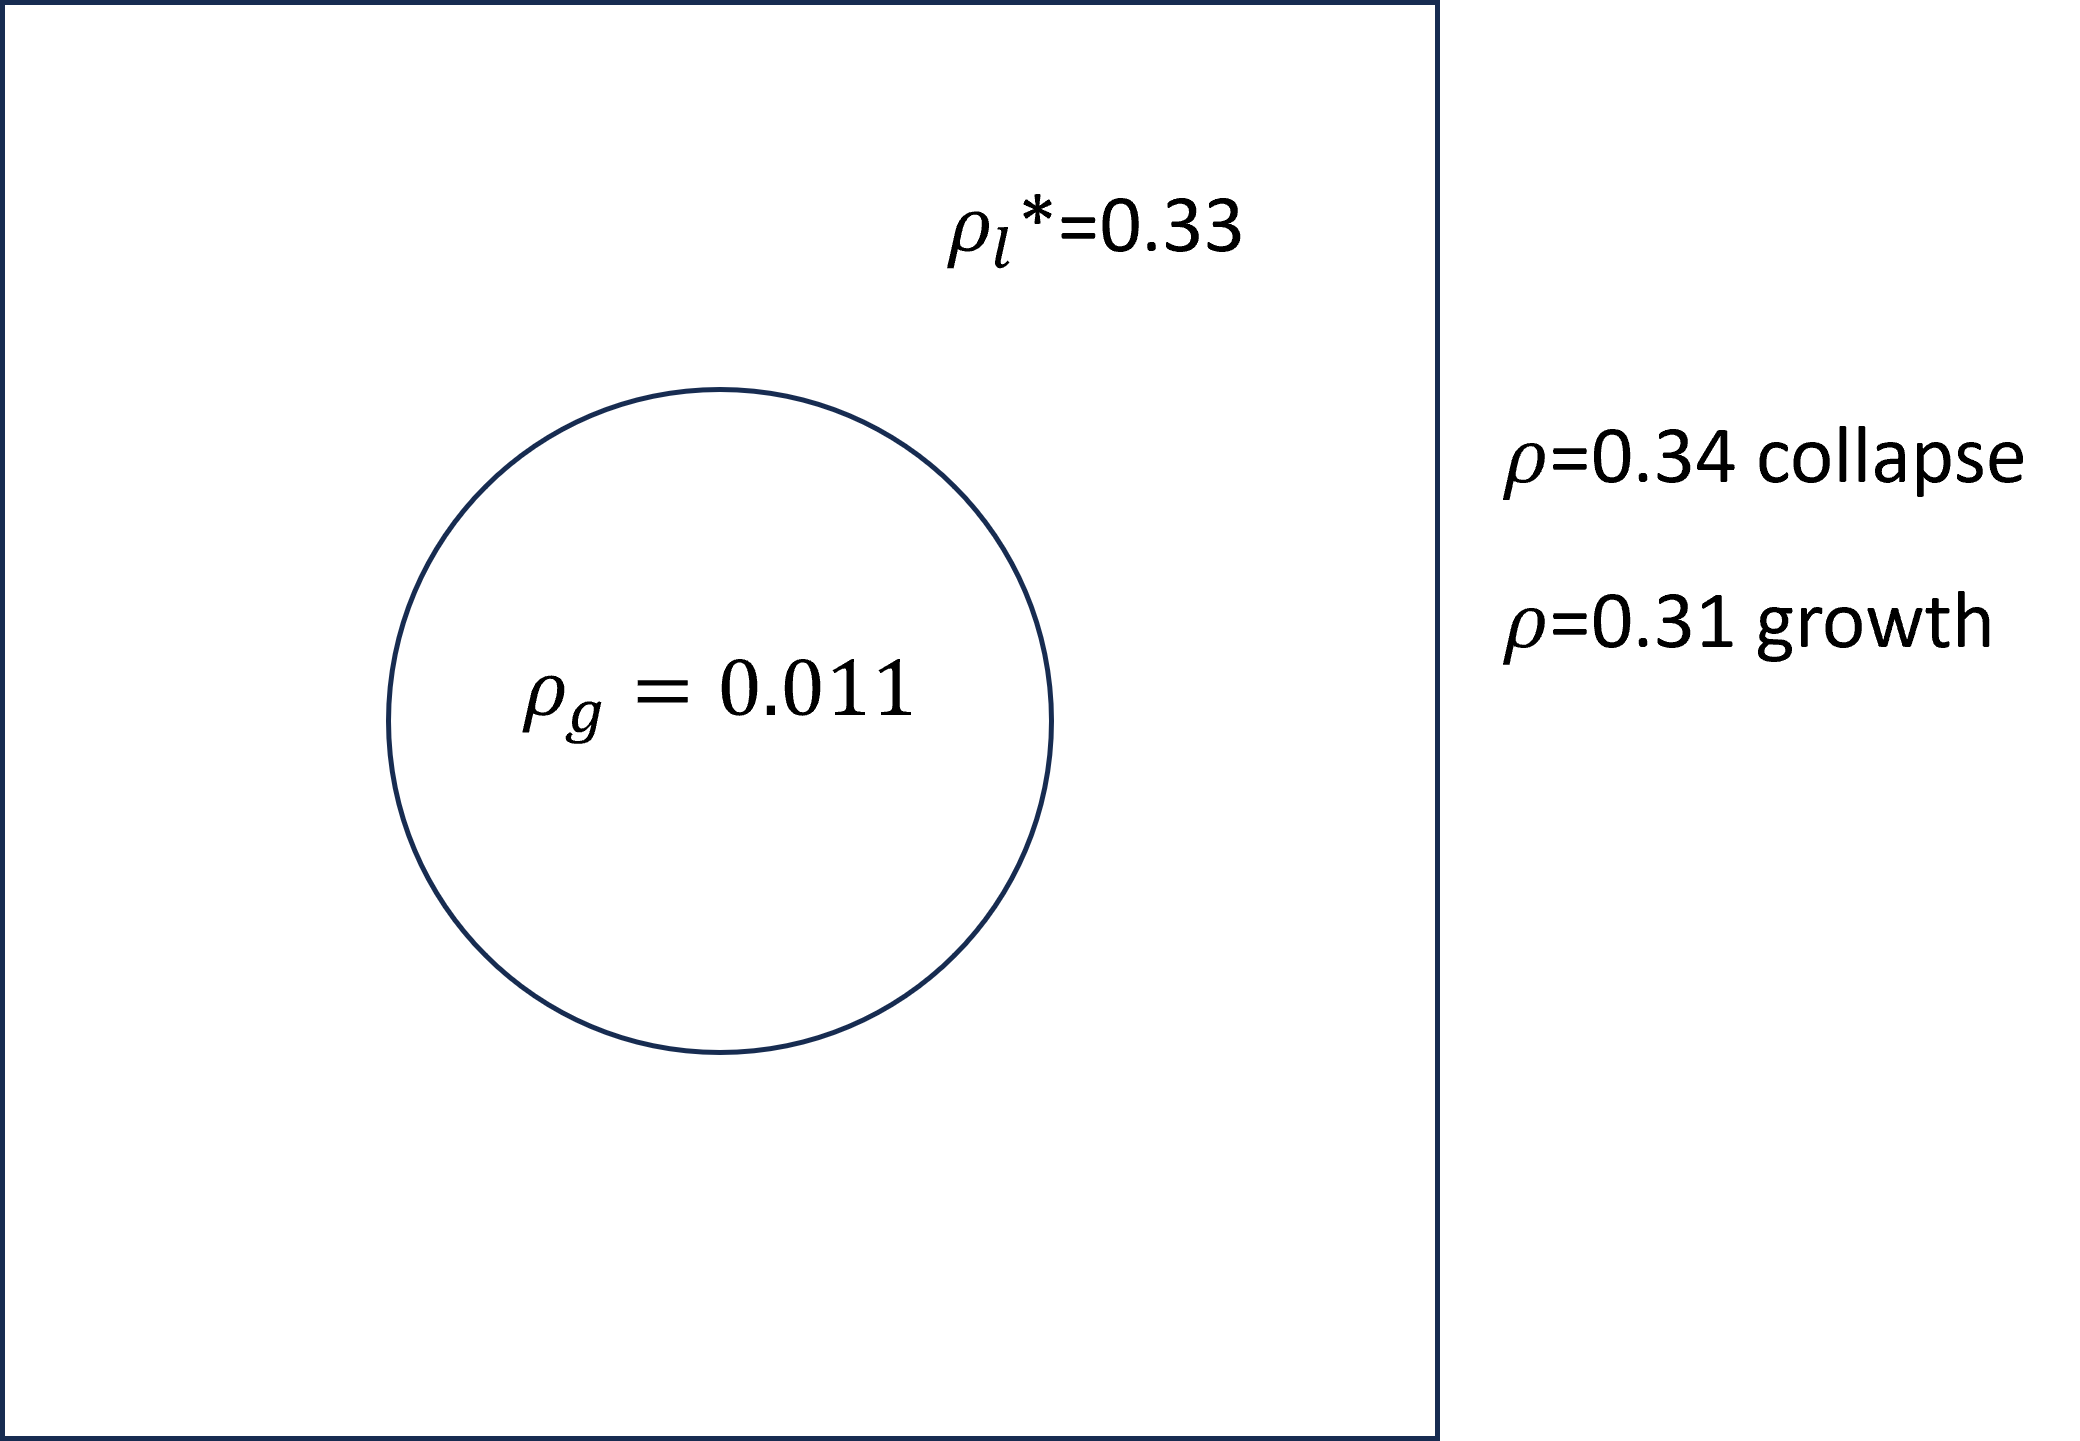
\includegraphics[width=0.7\textwidth]{schematic}
	\caption{schematic of the problem}
	\label{fig:schematics}
\end{figure}
In terms of the validation of Maxwell area construction, a flat interface simulation was performed to obtain the equilibrium density of liquid and gas according to Huang et al \cite{huang2019thermodynamic}. This is to validate the thermal consistency of the C-S equation of state. The reduced temperature in Maxwell area construction validation is from 0.55 to 1. As sketched in Figure \ref{fig:schematics-flat}, the gas is located in the middle with liquid around. To reach an equilibrium state of liquid and gas, the length of the domain is set to 20 lattice units and the height of the domain is set to 200 lattice units. In addition, the interfacial is also smoothed in flat interface simulation. After reaching the equilibrium state, the density of liquid and gas was kept against each reduced temperature. The equilibrium state is defined as when the density between two iterations is less than $1e^{-4}$.  

\begin{figure}[htp]
	\centering
	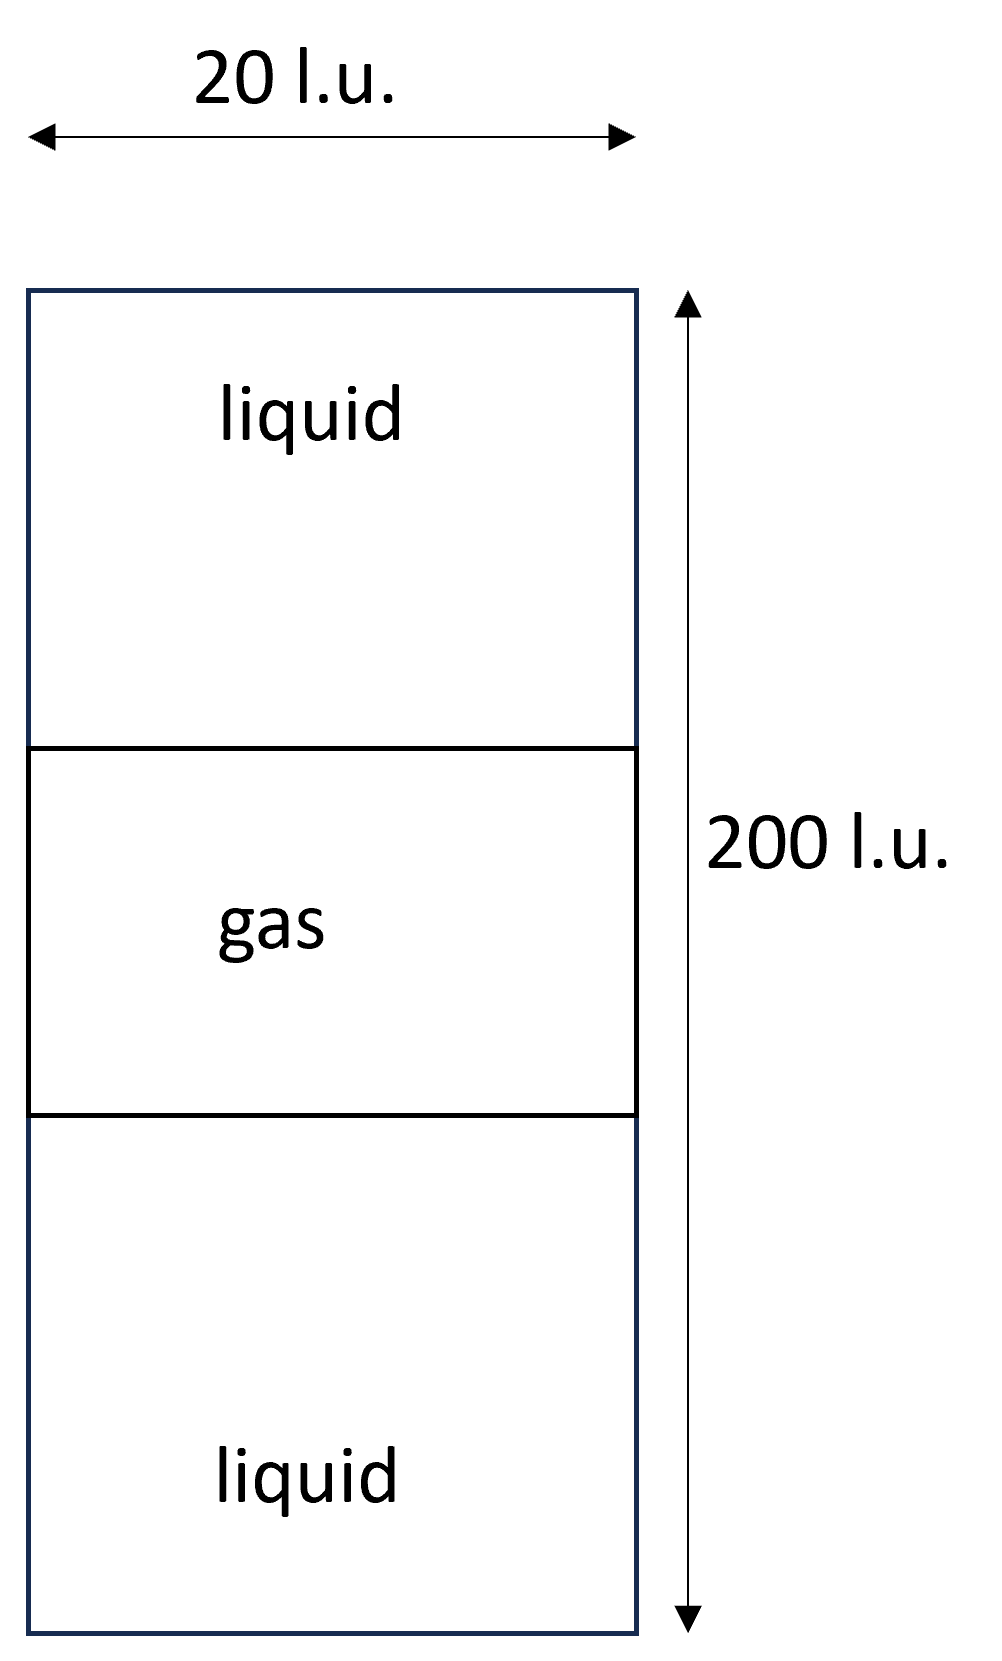
\includegraphics[scale=0.6]{flat-interface}
	\caption{schematic of the flat interface simulation}
	\label{fig:schematics-flat}
\end{figure}

To analyse the impact of domain size, radius and boundary condition, different cases were carried out as following table \ref{tab:cases}.
\begin{table}[ht]
	\centering
	\caption{different cases}
	\label{tab:cases}
	\begin{tabular}{c c c c c c}
		& & \\ % put some space after the caption
		\hline
		\hline
		density & Radius			&   	& domain size  				& 	& \\
		\hline
		0.31 &20			& 100  	& 200  				& 400	& 1000\\
		0.34 &20			& 100  	& 200  				& 400	& 1000\\
		0.31&		25			& 100  	& 200  				& 400	& 1000\\
		0.34&		25			& 100  	& 200  				& 400	& 1000\\
		0.31&30			& 100  	& 200  				& 400	& 1000\\
		0.34&30			& 100  	& 200  				& 400	& 1000\\
		0.31&35			& 100  	& 200  				& 400	& 1000\\
		0.34&35			& 100  	& 200  				& 400	& 1000\\
		\hline
		\hline
	\end{tabular}
\end{table}

As can be seen from the table \ref{tab:cases}, there are 32 cases total, each radius was performed two situation with growth and collapse and each situation was carried out with four domain size from 100 to 1000 domain size.    

\subsection{summary of SINDy algorithm}
To further analyse the deviation between the R-P equation and the LBM simulation, SINDy algorithm was used to identify the reasonable dynamic system. In this subsection, a brief summary of this algorithm is summarized here according to Bruton et al. \cite{brunton2017discovering}

In general,SINDy algorithm is used to identify the following equation \cite{brunton2017discovering},
\begin{linenomath}
	\begin{equation}
		\frac{d}{d t} \mathbf{x}(t)=\mathbf{f}(\mathbf{x}(t)),
	\end{equation}
\end{linenomath}
where $\mathbf{x}(t)$ is the temporary data that can be collected by any means such as experiment and simulation. $\mathbf{f}(\mathbf{x}(t))$ is the function that SINDy algorithm wants to identify with regression. Furthermore, $\mathbf{x}(t)$ can be expressed as a matrix with different states against time as follows \cite{brunton2017discovering},  
\begin{linenomath}
\begin{equation}
	\begin{gathered}
		\mathbf{X}=\left[\begin{array}{c}
			\mathbf{x}^T\left(t_1\right) \\
			\mathbf{x}^T\left(t_2\right) \\
			\vdots \\
			\mathbf{x}^T\left(t_m\right)
		\end{array}\right]=\left[\begin{array}{cccc}
			x_1\left(t_1\right) & x_2\left(t_1\right) & \cdots & x_n\left(t_1\right) \\
			x_1\left(t_2\right) & x_2\left(t_2\right) & \cdots & x_n\left(t_2\right) \\
			\vdots & \vdots & \ddots & \vdots \\
			x_1\left(t_m\right) & x_2\left(t_m\right) & \cdots & x_n\left(t_m\right)
		\end{array}\right]. \downarrow \text { time } \\
\end{gathered}
\end{equation}
\end{linenomath}
To obtain the derivative of $\mathbf{X}$, we can use numerical methods to calculate $\dot{\mathbf{X}}$ \cite{brunton2017discovering},
\begin{linenomath}
\begin{equation}
	\begin{gathered}
		\dot{\mathbf{X}}=\left[\begin{array}{c}
			\dot{\mathbf{x}}^T\left(t_1\right) \\
			\dot{\mathbf{x}}^T\left(t_2\right) \\
			\vdots \\
			\dot{\mathbf{x}}^T\left(t_m\right)
		\end{array}\right]=\left[\begin{array}{cccc}
			\dot{x}_1\left(t_1\right) & \dot{x}_2\left(t_1\right) & \cdots & \dot{x}_n\left(t_1\right) \\
			\dot{x}_1\left(t_2\right) & \dot{x}_2\left(t_2\right) & \cdots & \dot{x}_n\left(t_2\right) \\
			\vdots & \vdots & \ddots & \vdots \\
			\dot{x}_1\left(t_m\right) & \dot{x}_2\left(t_m\right) & \cdots & \dot{x}_n\left(t_m\right)
		\end{array}\right] .
	\end{gathered}
\end{equation}
\end{linenomath}
Then we can define different library which can be any candidate of any combination of $\mathbf{X}$ term as follows \cite{brunton2017discovering},
\begin{linenomath}
	\begin{equation}
		\Theta(\mathbf{X})=\left[\begin{array}{cccccccc}
			\mid & \mid & \mid & \mid & & \mid & \mid & \\
			1 & \mathbf{X} & \mathbf{X}^{P_2} & \mathbf{X}^{P_3} & \cdots & \sin (\mathbf{X}) & \cos (\mathbf{X}) & \cdots \\
			\mid & \mid & \mid & \mid & & \mid & \mid &
		\end{array}\right] .
	\end{equation}
\end{linenomath}
Once the library is defined and time series of data and numerical data is collected, following coefficient is determined by the SINDy algorithm \cite{brunton2017discovering}. 
\begin{linenomath}
\begin{equation}
	\Xi=\left[\begin{array}{llll}
		\boldsymbol{\xi}_1 & \boldsymbol{\xi}_2 & \cdots & \boldsymbol{\xi}_n.
	\end{array}\right]
\end{equation}
\end{linenomath}
In addition, to replicate the same terms of R-P equation, a constrained SR3 optimizer is used in this project which tries to minimize the following expression according to Kathleen et al\cite{champion2020unified} and Peng et al.\cite{zheng2018sparse}   
\begin{equation}
	\min _{\boldsymbol{x}, \boldsymbol{w}} \frac{1}{2}\|\mathbf{A} \boldsymbol{x}-\boldsymbol{b}\|^2+\lambda\|\boldsymbol{w}\|_1+\frac{1}{2 \eta}\|\boldsymbol{x}-\boldsymbol{w}\|^2
\end{equation}
To summarize, the SINDy algorithm aims to identify a general expression, as explained in \cite{brunton2017discovering}.
\begin{linenomath}
\begin{equation}
	\dot{\mathbf{X}}=\Theta(\mathbf{X}) \Xi.
\end{equation}
\end{linenomath}

\section{Results and Discussion}
\subsection{Laplace Law validation}
As stated before in the previous section, Laplace law validation was first performed with three initial radii. As can be seen from Figure \ref{fig:lap-law} (a),(b),(c), the bubble gradually evolve to the equilibrium state with periodic boundary condition. According to literatures \cite{porter2012multicomponent,liu2010modified,ezzatneshan2021dynamics} doing this validation, the Laplace Law can be expressed as
\begin{linenomath}
\begin{equation}
	p_c=p_b-p_s=\frac{\sigma}{R},
	\label{equ:lap}
\end{equation}
\end{linenomath}
where $\sigma$ is the surface tension,$R$ is the radius, and $p_c, p_b,p_s$ are the capillary pressure, bubble and suspending fluid pressure respectively. As can be seen from the figure \ref{fig:lap-law} (d), the results from LBM are quite agree with the Laplace law. The slope is the surface tension as expressed in Equation \ref{equ:lap}.
\begin{figure}[htp]
	\centering
	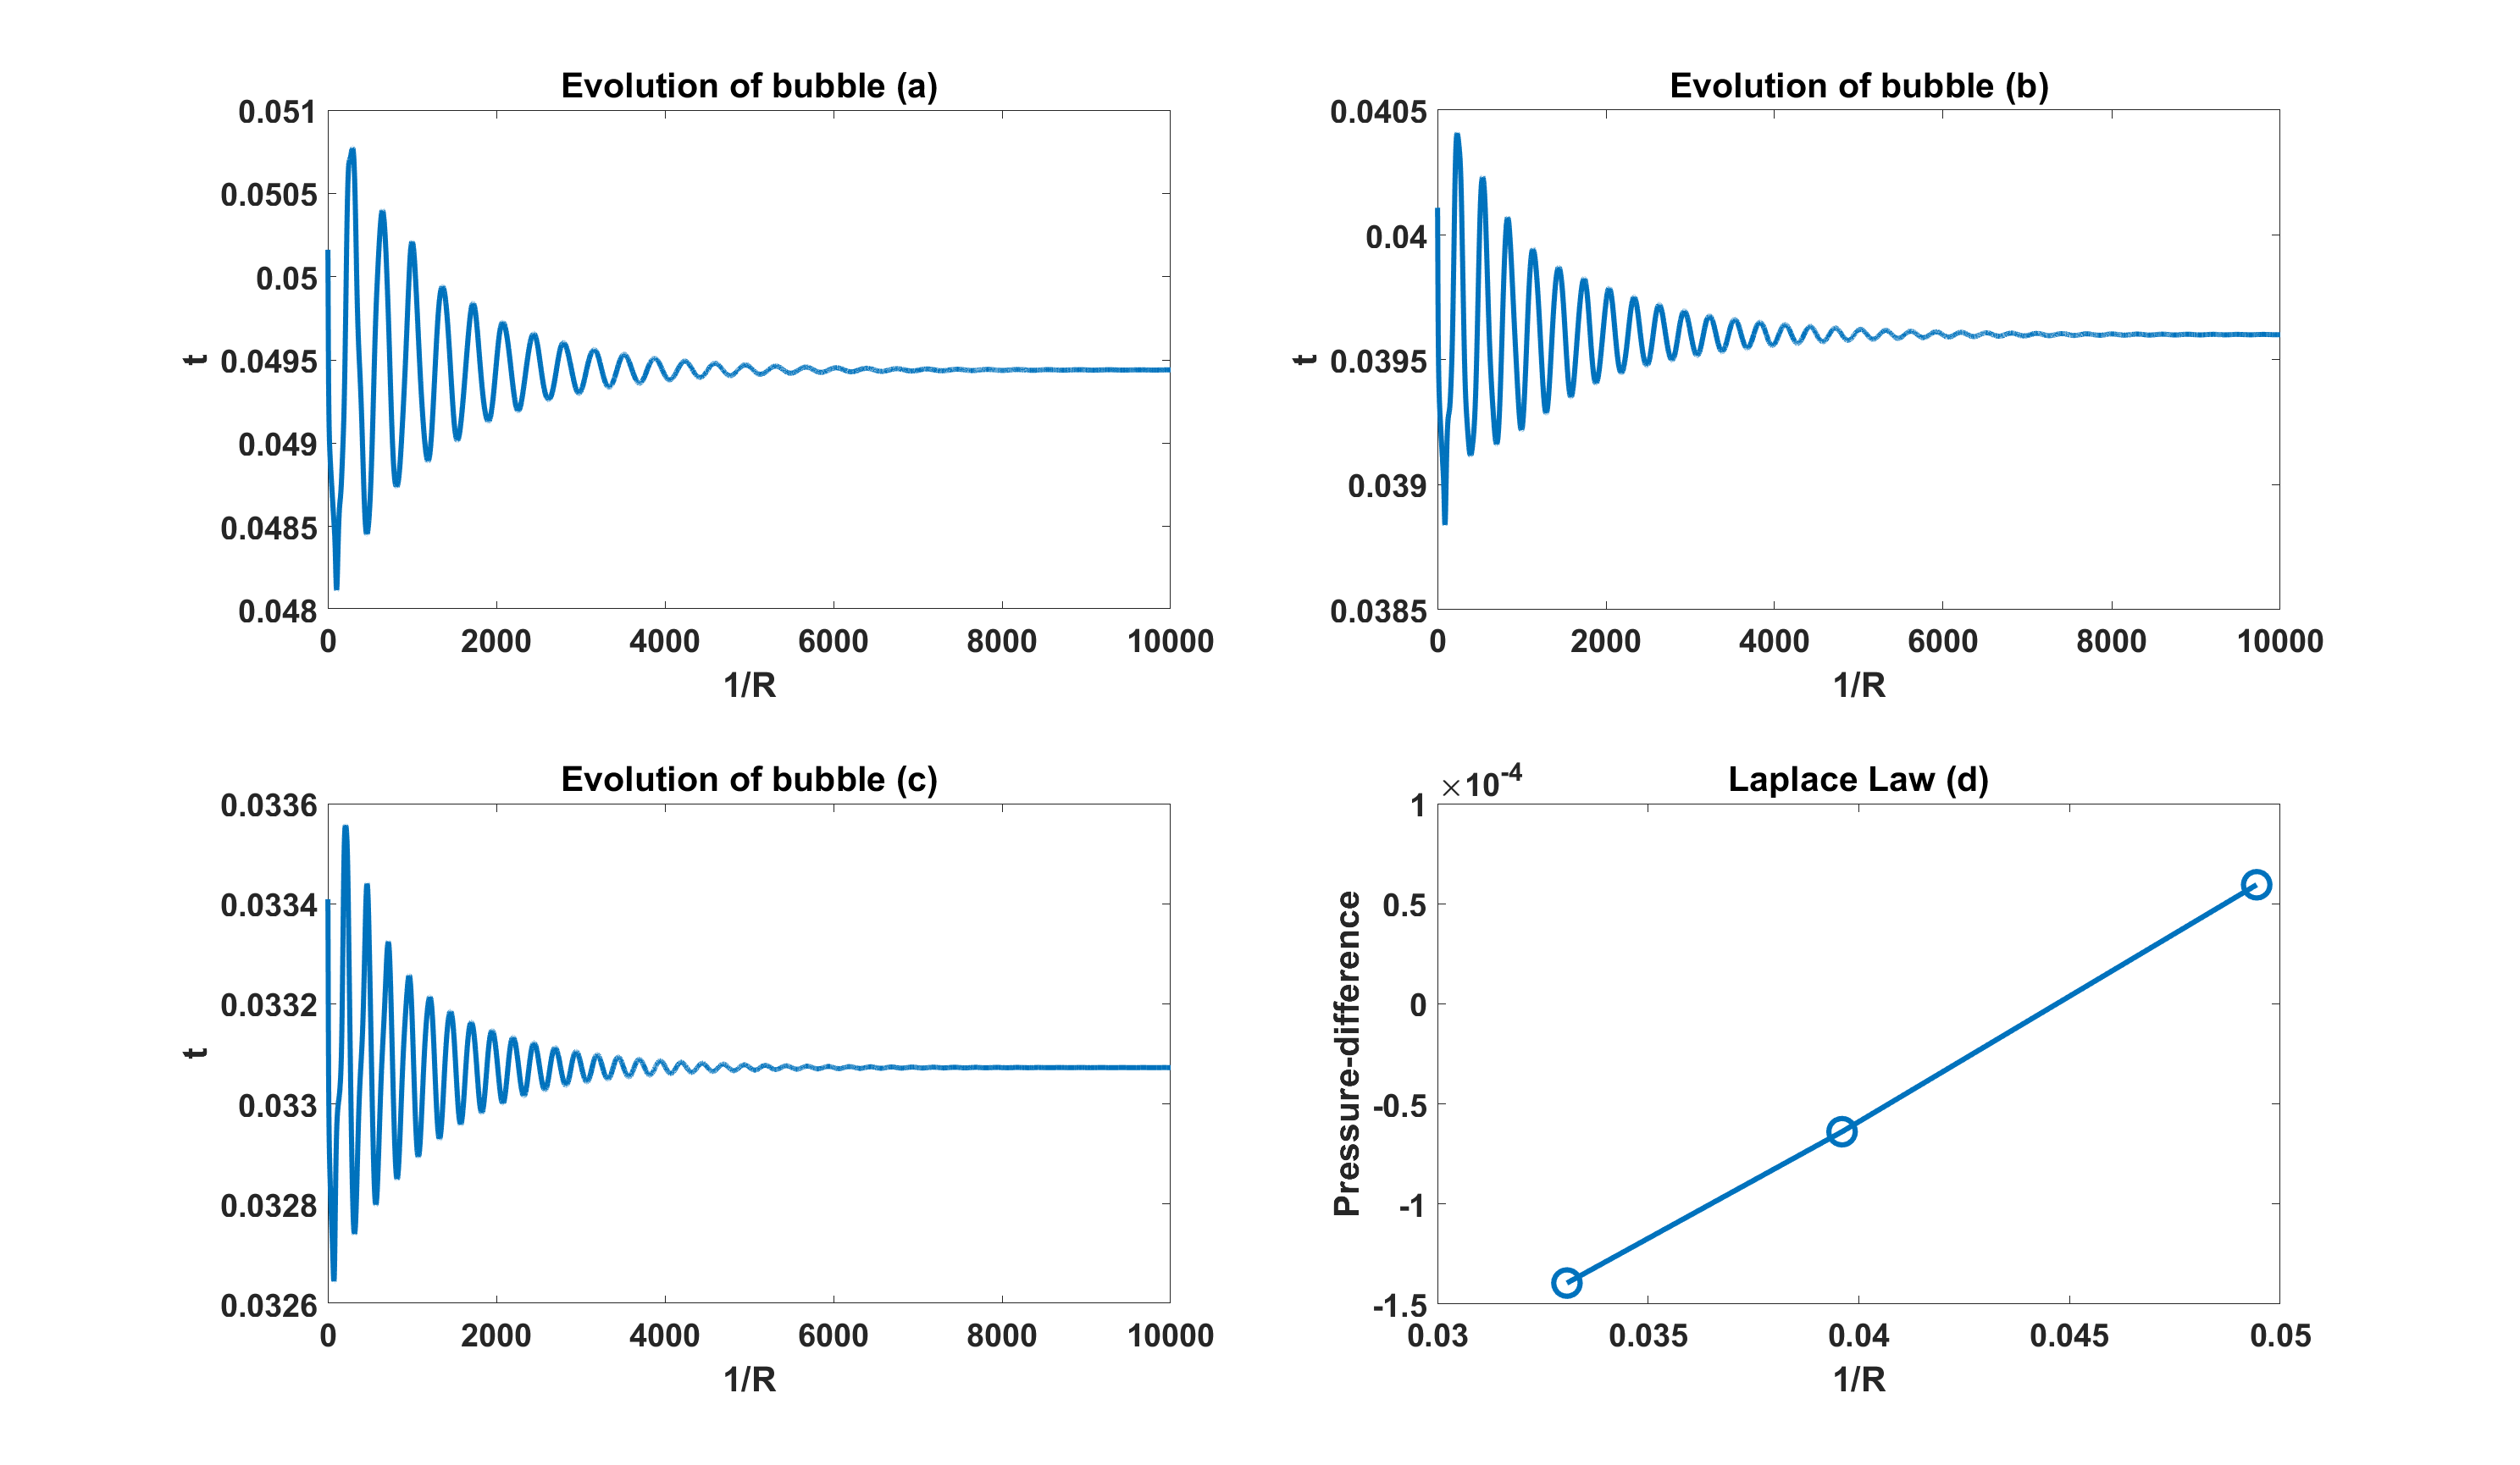
\includegraphics[width=1\textwidth,height=0.5\textheight]{laplacelaw-mat}
	\caption{Laplace Law (a) the change of radius of 20 initial bubble radius with time (b)the change of radius of 25 initial bubble radius with time (c) the change of radius of 30 initial bubble radius with time (d) Laplace law of pressure against reverse of radius }
	\label{fig:lap-law}
\end{figure}
\newpage
\subsection{Maxwell area construction validation}
As illustrated in the previous section, to validate the thermal consistency of the C-S equation of state, Maxwell area construction has to be performed. For the reason of simplicity, the reference data is digitized from Peng et al. \cite{peng2019simulation}. Figure \ref{fig:maxwell} shows the results of the equilibrium density of liquid and gas against different temperatures from a flat interface. It was shown that the LBM simulation has a good agreement with the Maxwell area construction, especially the equilibrium density of the liquid. There are some tiny discrepancies in the equilibrium gas density especially at low temperatures. This may be due to the fact that the numerical error and truncation error exist for the gas density. 
\begin{figure}[htp]
	\centering
	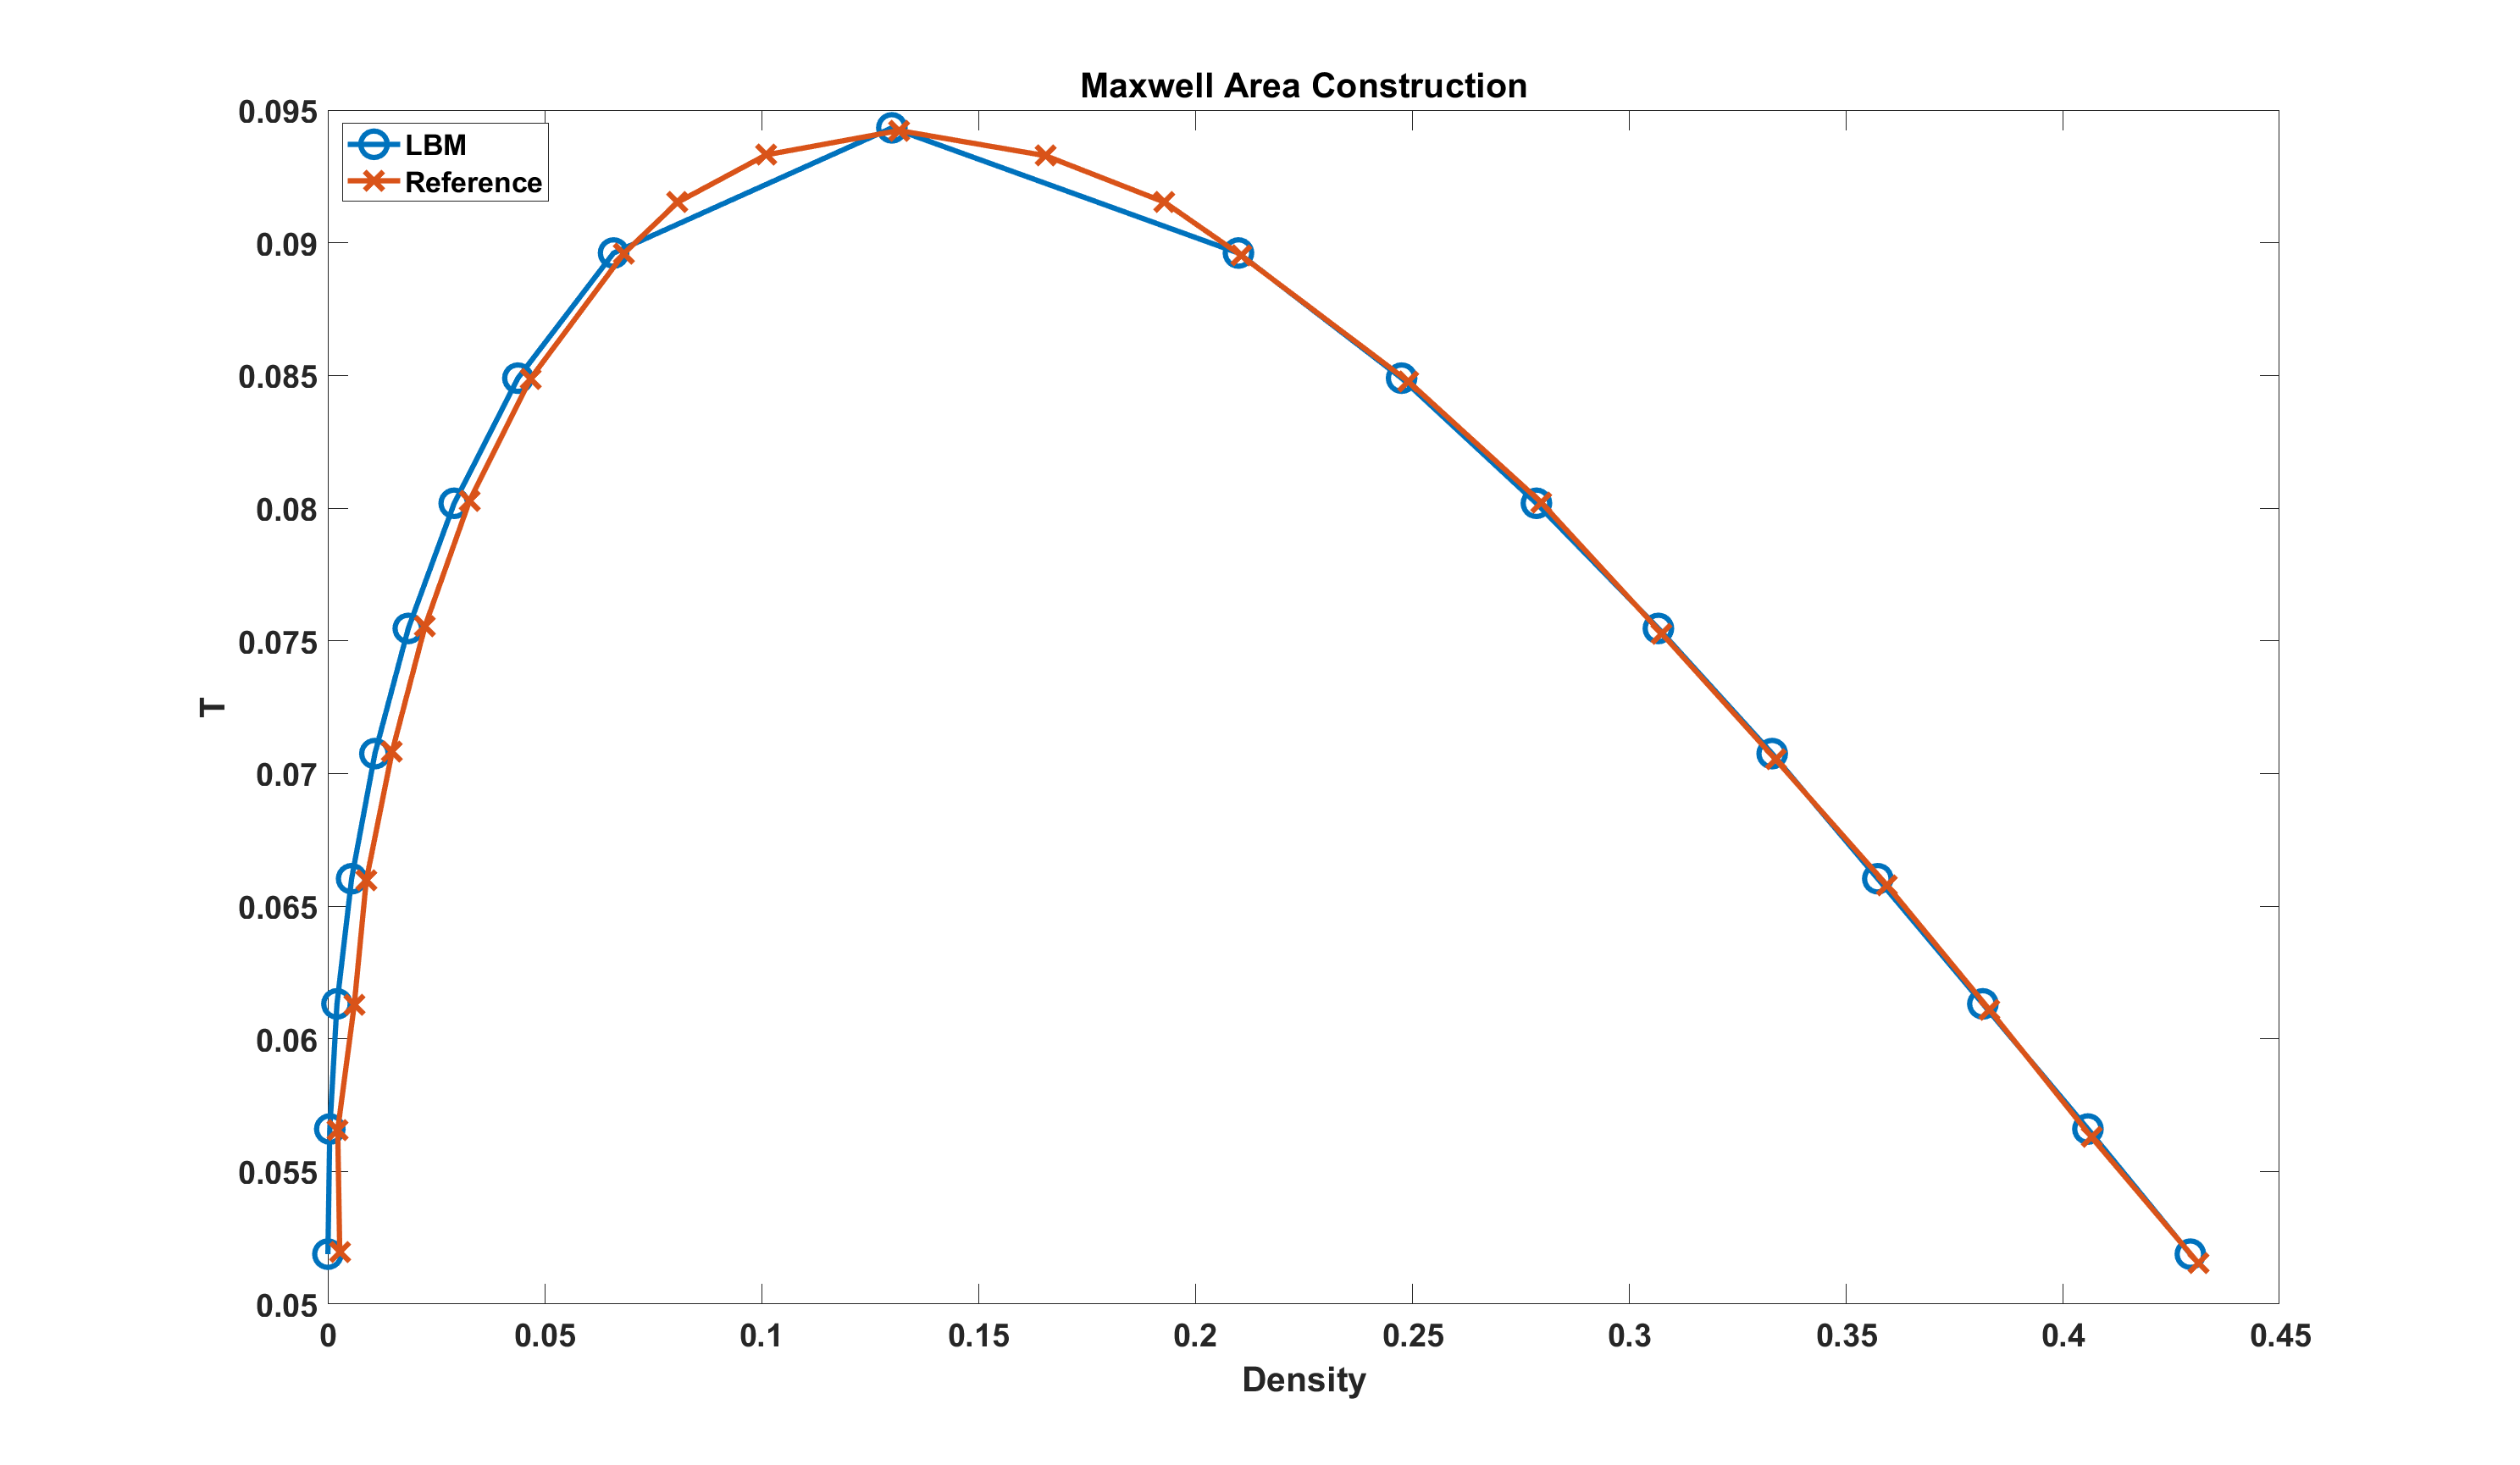
\includegraphics[width=1\textwidth,height=0.5\textheight]{maxwell}
	\caption{Maxwell area construction}
	\label{fig:maxwell}
\end{figure}
\subsection{growth and collapse curve}
Figure \ref{fig:bubble} shows different cases with different radii and domain sizes. As illustrated before, a validation of R-P against LBM is performed. Because LBM simulation is a two-dimensional square in this project. The R-P equation is derived from the cylinder-coordinated continuity and momentum equation. To solve the R-P equation, the Runge-Kutta ode45 solver of MATLAB was used. Figure \ref{fig:bubble} (a) (b) (c) (d) shows the growing cases with 100,200,400,1000 domain size with radius 20,25,30,35. It was important to note that the LBM simulation results were started from 100 iterations due to the fact it was not stable at the beginning of the simulation. As shown in the results of Peng et al. \cite{peng2019simulation}, at the beginning, there are always some discrepancies between LBM and the R-P equation. The results showed that with a beginning of 100 iterations, the match is good at the beginning, in this article we mainly focus on the other factors which impact the results, thus for simplicity, we begin at 100 iterations.  In addition, there are some distortions of the R-P equation with 100 and 200 domain sizes because when the bubble reaches the boundary, it cannot be solved correctly. There are mainly two results that can be found. Firstly, the LBM results start to deviate from certain iterations against the R-P solution. Secondly, with the increase of domain size, the iterations where it starts deviate increase, which will be analysed in the next subsection by chart. The same findings can be seen in the collapse case in figure \ref{fig:bubble} (e) (f) (g) (h). The radius to be negative for R-P in 200 domain size is because there is no limit for the R-P equation. 


\subsection{The Analysis of Iterations and Radius for Achieving 5\% Deviation}
The findings are further analysed on the chart in this subsection. Figure \ref{fig:chart} (a) (b) shows the iterations when the deviation between LBM and R-P is greater than 5\%. With the increase of domain size, the iterations within 5\% error increase for each radius. However, with domain size 100 with 20 radius there is a difference. The reason for that may be due to the low resolution with a small radius. Within the same domain size, the iterations within 5\% error almost increase with the increase of radius except for the 100 domain size with 20 radius. And, there are slight decreases for domain size 400 and 1000 from 25 to 30. The boundary condition affects the simulation of LBM with non-physical wave which has less impact when the domain size increases. In the 1000 domain case, the error within 5\% even reaches 1000, which again proves that when the domain size is large enough, the non-physical wave can be neglected. In terms of the collapse case, a similar phenomenon can be seen, with the increase of domain size, the iterations within 5\% error increase for each radius except the 100 domain size case. This is also true that the iterations within 5\% error almost increase with the increase of radius except the 100 domain size with 20 radius. When the domain size increases, the resolution in the bubble increases, which makes the iteration within 5\% error increase for the collapse cases. 
\begin{figure}[htp]
	\centering
	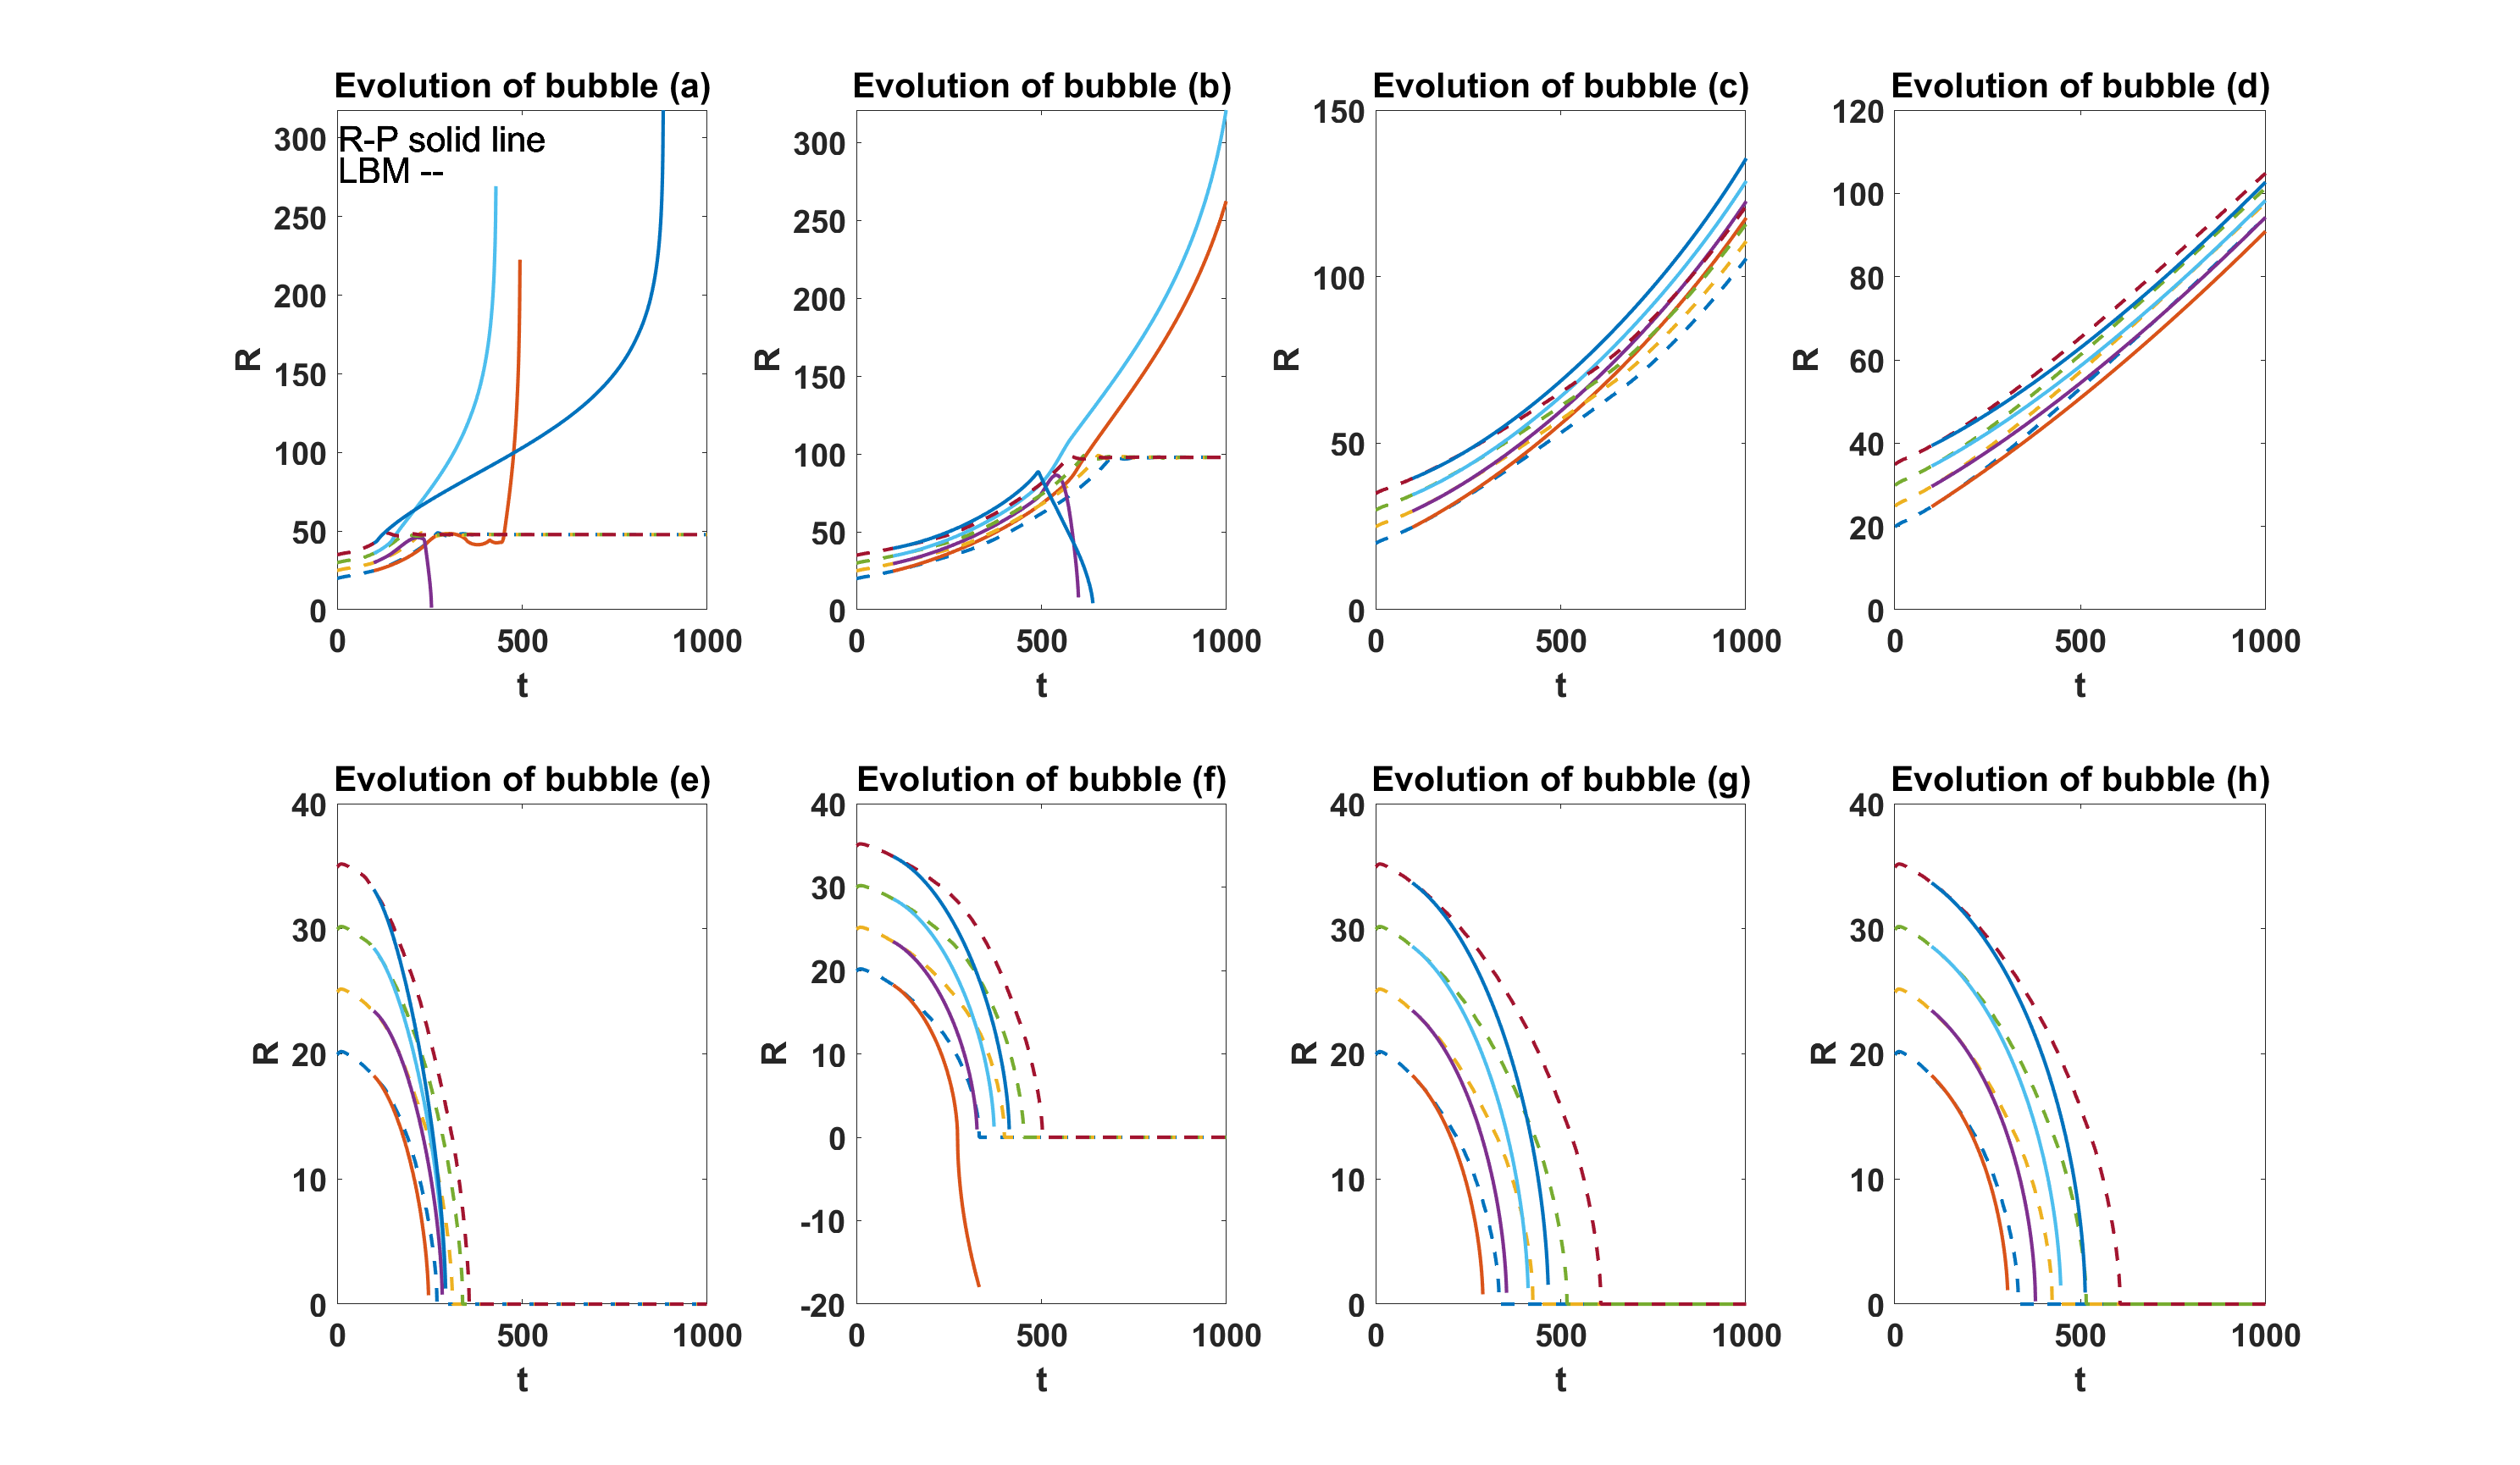
\includegraphics[width=1\textwidth,height=0.5\textheight]{bubble-curve}
	\caption{different cases, (a)-(d) growth cases with domain size 100,200,400,1000, (e)-(h) collapse cases with domain size 100,200,400,1000. Each case display the results of radius 20,25,30,35. }
	\label{fig:bubble}
\end{figure}
With the increase of the domain size, the radius within 5\% error increases for each domain size except the 100 domain size case with 20 radius. There are slight decrease for the radius of 25 from 400 domain size to 1000 domain size. In addition, within the same domain size, the radius within 5\% error also increases except in 100 domain size case with a radius of 20 and 1000 domain size with a radius of 25. 
A similar phenomenon can be seen in collapse cases, especially within the same domain size, the radius within 5\% error also increases without any exception. In addition, within the same domain size, the radius within 5\% error also decreases except in 100 cases. This also suggests that for the growth case, the boundary condition also has an impact on the accuracy of the LBM simulation with a non-physical wave, with the increase of the domain size, the wave has more time to return from the boundary which will affect the radius of the bubble.
 
\begin{figure}[htp]
	\centering
	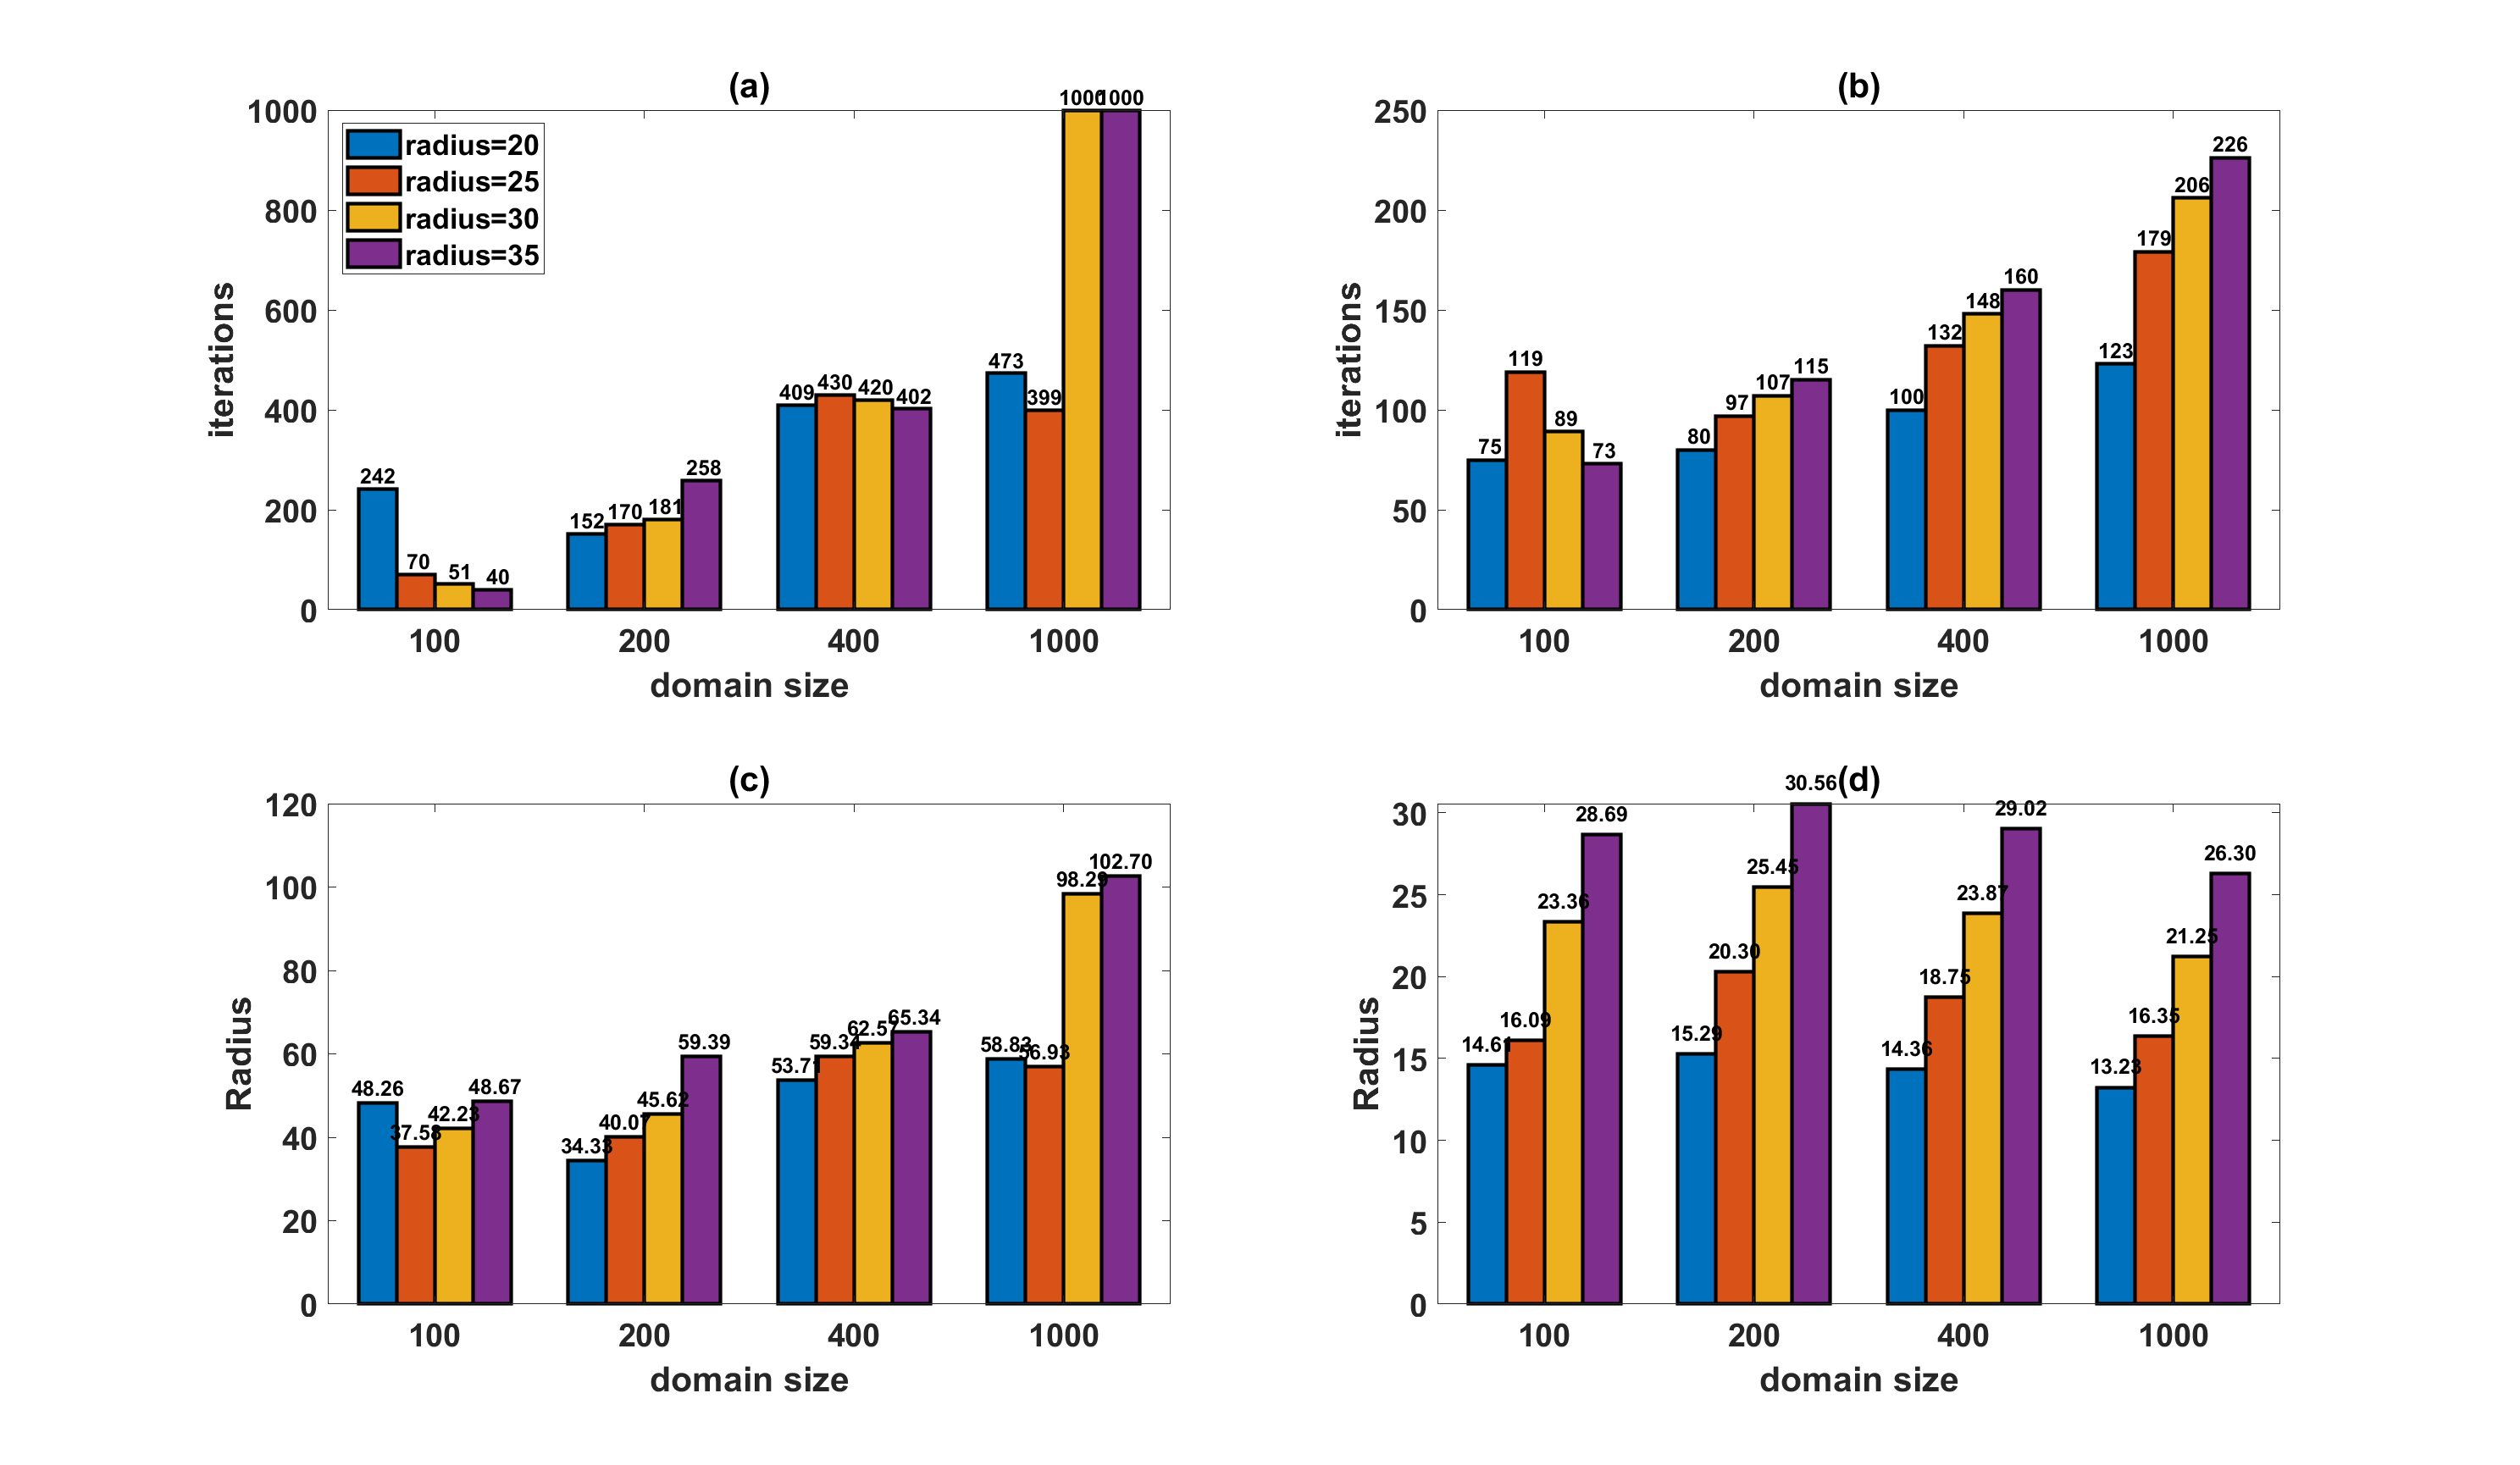
\includegraphics[width=1\textwidth,height=0.5\textheight]{chart}
	\caption{different cases when the deviation greater than 5\%. (a) iterations when deviation greater than 5\% of growth cases, (b) iterations when deviation greater than 5\% of collapse cases, (c) radius when deviation greater than 5\% of growth cases, (d) radius when deviation greater than 5\% of collapse cases }
	\label{fig:chart}
\end{figure}
In terms of the collapsing case, with the increase of domain size, the resolution of the radius will increase which increases the radius reaching 5\% error. In both cases, the 100 domain size is the exception case which may be due to the fact that the resolution is not large enough for the collapse case and the bubble is so susceptible to the boundary wave.

\subsection{SINDy}
In the previous subsection, it has been proved that the R-P equation is not perfect for LBM bubble simulation validation. Thus in this subsection, SINDy algorithm is used to better fit the LBM simulation and offer a new equation for this bubble evolution. As stated before, the R-P equation is as equation \ref{equ:r-p},thus there are the following terms,
\begin{linenomath*}
	\begin{equation}
		\frac{c 1}{R \ln \frac{c 7}{R}}, \frac{c 2}{R^2 \ln \frac{c 7}{R}}, \frac{c 3 \dot{R}}{R^2 \ln \frac{c 7}{R}}, \frac{c4\dot{R}^2}{2 * R \ln \frac{c 7}{R}}, \frac{c5 R \dot{R}^2}{c 7^2 2 \ln \frac{c 7}{R}}, \frac{c6 \dot{R}^2}{R}.
	\end{equation}
\end{linenomath*}
where $c1,c2,c3,c4,c5,c6,c7$ are constant. In this article, the same terms of R-P equation are fed to SINDy customised library. In addition, the same coefficient of R-P is also implemented for the initial guess of SINDy. Figure \ref{fig:sindy-100} and \ref{fig:sindy-1000} depict the results of SINDy customised library and polynomial library within different iterations. In this section, 100 and 1000 domain size are studied based on SINDy. Figure \ref{fig:sindy-100} are the results of 100 domain size and Figure \ref{fig:sindy-1000} are the results of 1000 domain size. As can be seen in figure \ref{fig:sindy-100} (a),(b),(c), the iterations from 70 to 210 have better results than the other two. This may be due to the fact that at the beginning, there is some noise. In addition, if the data contains too little, the regression of SINDy may not have good results. The same thing can be found in the collapse case in Figure \ref{fig:sindy-100} (d),(e),(f), where the results within iterations from 100 to 300 have better results. For both the growth case and collapse case, results after certain iterations are also not convincing because for the growth case, the bubble reaches the boundary and the bubble disappears for the collapse case. Figure \ref{fig:sindy-1000} also demonstrates that the results of SINDy customised library have better results in the middle range of iterations. 

\begin{figure}[htp]
	\centering
	\includegraphics[scale=0.25]{SINDy-100}
	\caption{SINDy regression results with R-P customised library and polynomial library (a) (b) (c) domain size=100,growth case,radius=25,(d) (e) (f) domain size=100,collapse case,radius=25, (a) iterations from 30 to 210, (b) iterations from 70 to 210, (c) iterations from 110 to 210, (d) iterations from 60 to 300, (e) iterations from 100 to 300, (f) iterations from 150 to 210  }
	\label{fig:sindy-100}
\end{figure}
\begin{figure}[htp]
	\centering
	\includegraphics[scale=0.25]{SINDy-1000}
	\caption{SINDy regression results with R-P customised library and polynomial library (a) (b) (c) domain size=1000,growth case,radius=25,(d) (e) (f) domain size=1000,collapse case,radius=25, (a) iterations from 15 to 250, (b) iterations from 150 to 250, (c) iterations from 150 to 290, (d) iterations from 15 to 250, (e) iterations from 100 to 250, (f) iterations from 150 to 420 }
	\label{fig:sindy-1000}
\end{figure}

\newpage
To better understand and compare SINDy with R-P equation, table \ref{tab:SINDy-cases} is summarized with different cases for the coefficient that SINDy obtained.  
\begin{table}[ht]
	\centering
	\caption{coefficient of SINDy with different cases}
	\label{tab:SINDy-cases}
	\small
	\begin{tabular}{c c c c c c c}
		& & \\ % put some space after the caption
		\hline
		\hline
		\makecell{Iterations,\\domain size,\\case} & \makecell{c1(0.0158 growth or\\ -0.0065 collapse) }& \makecell{c2 (-0.0707 growth or \\-0.0645 collapse) } & \makecell{c3\\(-0.333)} & \makecell{c4\\ (1) } & \makecell{c5\\ (-1)} & \makecell{c6\\ (-1) } \\
		\hline
		30-210,100,growth &0.018(13.92\%)			& -0.087(23.06\%)  	& -0.329  				& 1.031	& -0.974&-0.996\\
		70-210,100,growth &0.019(20.25\%)			& -0.073(3.25\%) 	& -0.332  				& 1.014	& -0.985&-1.002\\
		110-210,100,growth&		0.016(1.27\%)			& -0.097(37.20\%)  	& -0.330  				& 1.041	& -0.961&-1.002\\
		60-300,100,collapse&		-0.008(23.08\%)			& -0.016(75.20\%)  	& -0.352  				& 1.012	& -1.000&-0.936\\
		100-300,100,collapse&-0.010(53.85\%)		& -0.004(93.80\%)  	& -0.355 				& 1.014	& -1.000&-0.930\\
		150-210,100,collapse&-0.004	(38.46\%)		& -0.072(11.63\%)  	& -0.333  				& 1.000	& -1.000&-1.000\\
		15-250,1000,growth&0.018(13.92\%)			& -0.071(<1\%) 	& -0.333  				& 1.000	& -1.000&-1.000\\
		150-250,1000,growth&0.027(70.89\%)			& -0.070 (<1\%) 	& -0.333  				& 1.000	& -1.000&-1.000\\
		150-290,1000,growth&0.019(20.25\%)			& -0.071(<1\%)  	& -0.333  				& 1.000 	& -1.000 &-1.000 \\
		15-250,1000,collapse&-0.007(7.70\%)		& -0.072(11.63\%)  	& -0.333  				& 1.000	& -1.000&-1.000\\
		100-250,1000,collapse&-0.005(23.08\%)			& -0.072(11.63\%)  	&-0.333  				& 1.000	& -1.000&-1.000\\
		150-420,1000,collapse&0.012	(284.62\%)		& -0.116(79.84\%) 	& -0.307 				& 0.991	& -1.000&--1.000\\
		\hline
		\hline
	\end{tabular}
\end{table}
As can be seen from table \ref{tab:SINDy-cases}, the coefficient obtained by SINDy is very close to R-P equation, especially c3,c4,c5, and c6, which are all less than 10\%. The difference between the c1 and c2 coefficient of R-P and SINDy is almost less than 50\% except in some cases. It is found that there is no connection between the difference in coefficient and the close of SINDy results with LBM data. It is also demonstrated that within iterations from 150 to 420 with 1000 domain size, the sign of the c1 coefficient is different than the R-P equation. In Figure \ref{fig:sindy-1000} (f), after certain iterations, the deviation between SINDy and LBM data increases which is related to the wrong prediction of the c1 coefficient.  
\section{Conclusions}
This article performed the LBM simulation of a single bubble based on the Shan-Chen Model. Then validate the results with R-P equation and try to replicate R-P based on SINDy algorithm. Based on the previous results and discussion, the following results can be drawn,
\begin{itemize}
	\item First of all, Laplace law and Maxwell's area construction are validated before R-P equation validation.
	\item From the comparison of the R-P results and LBM, there are deviations from certain iterations. In addition, the iterations where deviation starts to increase become larger with the increase of the domain size. 
	\item The analysis from the chart also shows that with the increase of domain size for each radius, the iterations where deviation larger than 5\% increase expect the 100 domain size in both collapse and growth cases.
	\item The analysis from the chart also shows that with the increase of radius for each domain size, the iterations where deviation larger than 5\% increase expect some special cases in both collapse and growth cases.
	\item The radius where deviation larger than 5\% also increases with the increase of domain size except the 100 domain size due to the fact that resolution of 100 domain size is not high enough. 
	\item The deviation exists because after certain iterations, in terms of the growth bubble, the impact of the boundary starts to become important. In terms of collapse cases, after certain iterations, the resolution is not big enough for the calculation of the bubble radius.
	\item With the same terms of R-P and initial guess of the coefficient of R-P, SINDy can provide good results within certain iterations in the middle. There is some noise at the beginning of the LBM data and the end, which is the same as the results of the validation of R-P against LBM.
\end{itemize}

\section*{Acknowledgements}
This project was financially supported by the Centre for Computational Engineering Sciences at Cranfield University under project code 15124. Furthermore, we would like to acknowledge the IT support for using the High-Performance Computing (HPC) facilities at Cranfield University, UK.
%\appendix
%\section{some appendix}\label{app:A}


%\section*{References}

{\begingroup
\singlespacing
\footnotesize
\bibliography{mybibliography}
\endgroup}

\end{document}